
% = SECTION =
\section{An analysis of DDGMs \label{sec:analysis}}

The core idea behind DDGMs is the gradual noise injection to images as we go forward in time such that the final object is a sample from the standard Gaussian distribution. Then, in the backward diffusion process model reverts this procedure and, as a result, generates new objects. Therefore, understanding the success of DDGMs relies heavily on understanding how the injected noise influences the behavior of both training and the model itself.

\paragraph{The noise distribution in the forward diffusion process} The first question we ask is how much corrupted an image gets after applying a specific noise schedule. Following %other work (e.g., 
\cite{ho2020denoising, kingma2014autoencoding, nichol2021improved}, we can utilize the signal-to-noise ratio (SNR), expressed as the squared mean of a signal (here: image) divided by the variance of a signal, to quantify the amount of noise in $\rvx_t$. For this purpose, the quantity of interest is the forward diffusion for a given $\rvx_0$, namely, $q(\rvx_t | \rvx_0)$, that results in the following SNR:
\begin{equation}\label{eq:snr}
    SNR(\rvx_0, t) = \frac{\overline{\alpha}_t \rvx_0^2}{1 - \overline{\alpha}_t} .
\end{equation}

Similarly to \cite{kingma2021variational}, we formulate the forward diffusion in such a way that the SNR is strictly monotonically decreasing in time, namely, $SNR(\rvx_0, t) < SNR(\rvx_0, s)$ for $t > s$. This means that an image becomes more noisy as we go forward in time. 

\begin{figure}[h!]
	\centering
    \subfloat[Linear noise schedule]{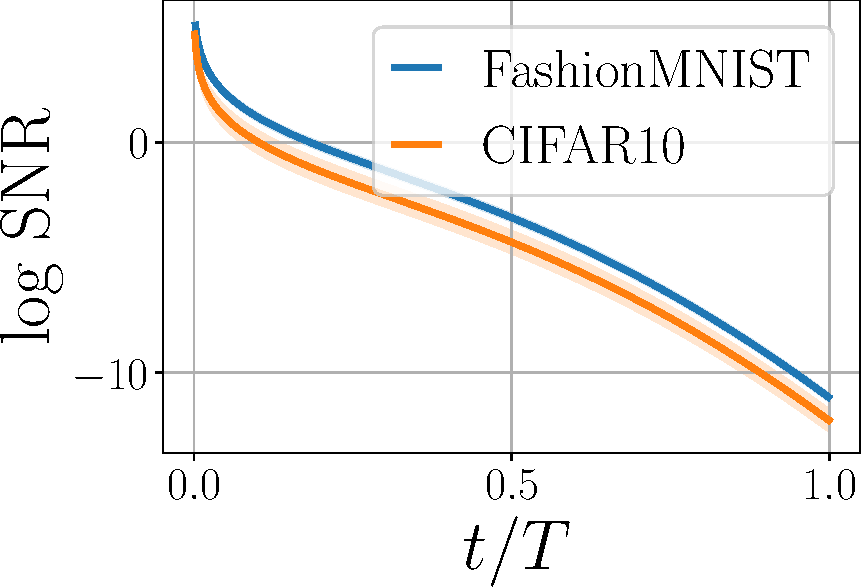
\includegraphics[width=0.34\linewidth]{pics/4_daed/snr/linear_0_1.0_snr_w.pdf}
    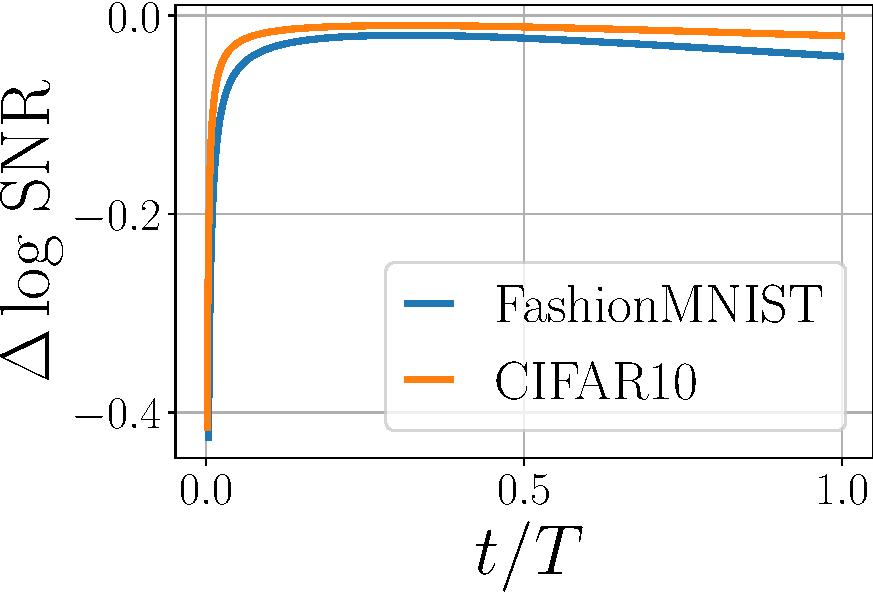
\includegraphics[width=0.34\linewidth]{pics/4_daed/snr/linear_0_1.0_delta_snr.pdf}}  \quad
    \subfloat[Cosine noise schedule]{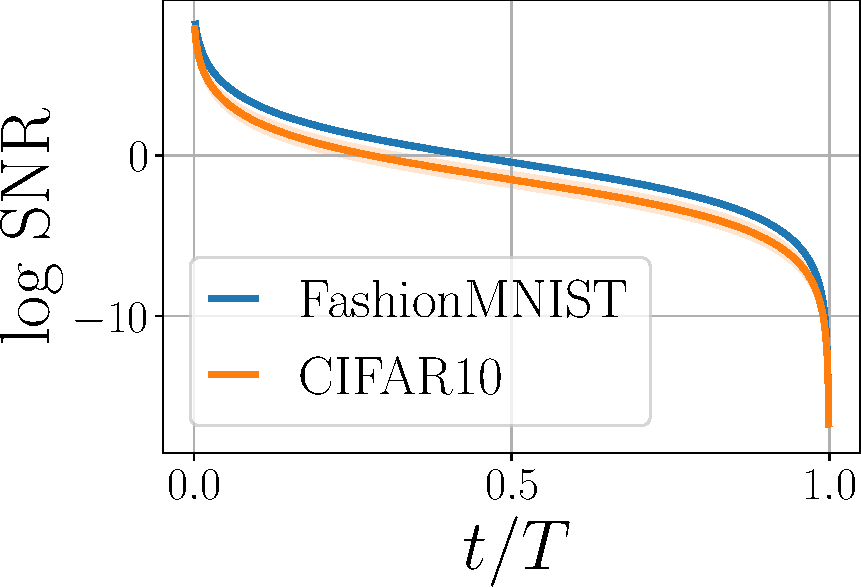
\includegraphics[width=0.34\linewidth]{pics/4_daed/snr/cosine_0_1.0_snr_w.pdf} 
    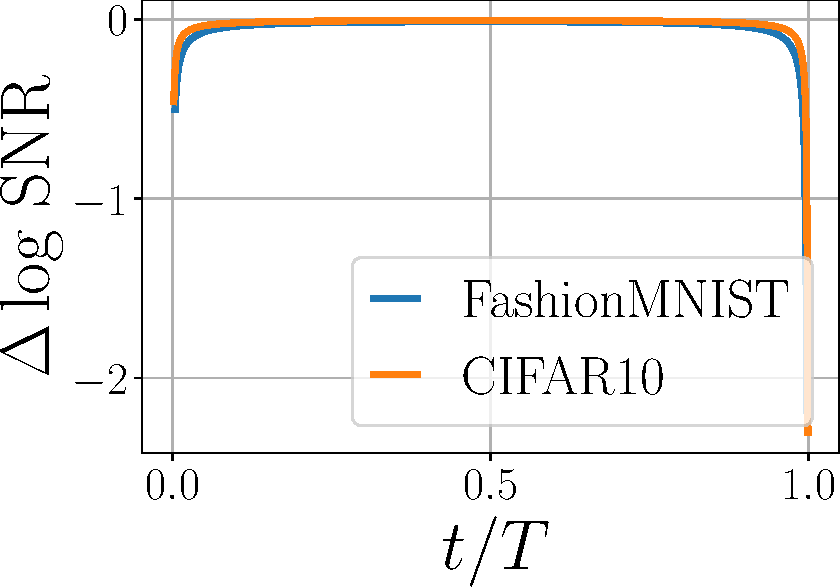
\includegraphics[width=0.34\linewidth]{pics/4_daed/snr/cosine_0_1.0_delta_snr.pdf}}
    % \vskip  -4pt
	\caption{Logarithm of the signal-to-noise ratio averaged over the dataset (solid line) and its standard deviation, and the difference of the $\log$ SNR within two consecutive time steps.}
	\label{fig:snr_analysis}
	\vskip  -4pt
\end{figure}

In Figure \ref{fig:snr_analysis} (left) we plot the logarithm of the SNR for both linear (Figure \ref{fig:snr_analysis}.a) and cosine (Figure \ref{fig:snr_analysis}.b) noise schedules for two datasets (FashionMNIST and CIFAR10). We average SNR over the $\rvx_0$'s (from the corresponding dataset). The right column depicts the change of the $\log$ SNR, i.e., its discrete derivative $\Delta \log \text{SNR}(t) = \log \text{SNR}(x_0, t) - \log \text{SNR}(x_0, t-1)$. First of all, we can notice a point at which the log-SNR drops below $0$. This corresponds to the situation of the noise overshadowing the signal. In the case of the linear noise schedule, this happens after about $20\%$ of steps, while for the cosine noise schedule, it appears after about $25-50\%$ of steps. However, the transition occurs in both cases. The biggest changes in the log-SNR are noticeable within the first $10\%$ of steps. This may suggest that the signal is the strongest within the first $10-20\%$ of the forward diffusion process steps, and then it starts being overshadowed by the noise. 

\paragraph{The reconstruction error of DDGMs} Since we know that the signal is not lost within the first $10-20\%$ of steps, the next question is about the reconstruction capabilities of DDGMs, namely, what is the reconstruction error of $\rvx_t \sim q(\rvx_t | \rvx_0)$. To be clear, we are not interested in how much each step of a DDGM contributes to the final objective (e.g., see Figure 2 in \cite{nichol2021improved}) but rather how well a DDGM reconstructs a noisy image $\rvx_t$.
In Figure \ref{fig:reconstruction_error_analysis} we plot the \textit{Mean Absolute Error} (MAE) and the \textit{Multi-Scale Structural Similarity} (MS-SSIM) \cite{wang2003multiscale} that both measure the difference between an original image $\rvx_0$ and a corrupted image at the $t^{th}$ step $\rvx_t$ reversed by the backward diffusion. 

%\begin{wrapfigure}{r}{0.57\textwidth}
%% \vskip  -11pt
%    \begin{adjustbox}{center}
     \begin{figure}[t]
    \begin{tabular}{cc}
    %   $\log$ SNR $(t)$ &  $\Delta$ $\log$ SNR $(t)$ \\
        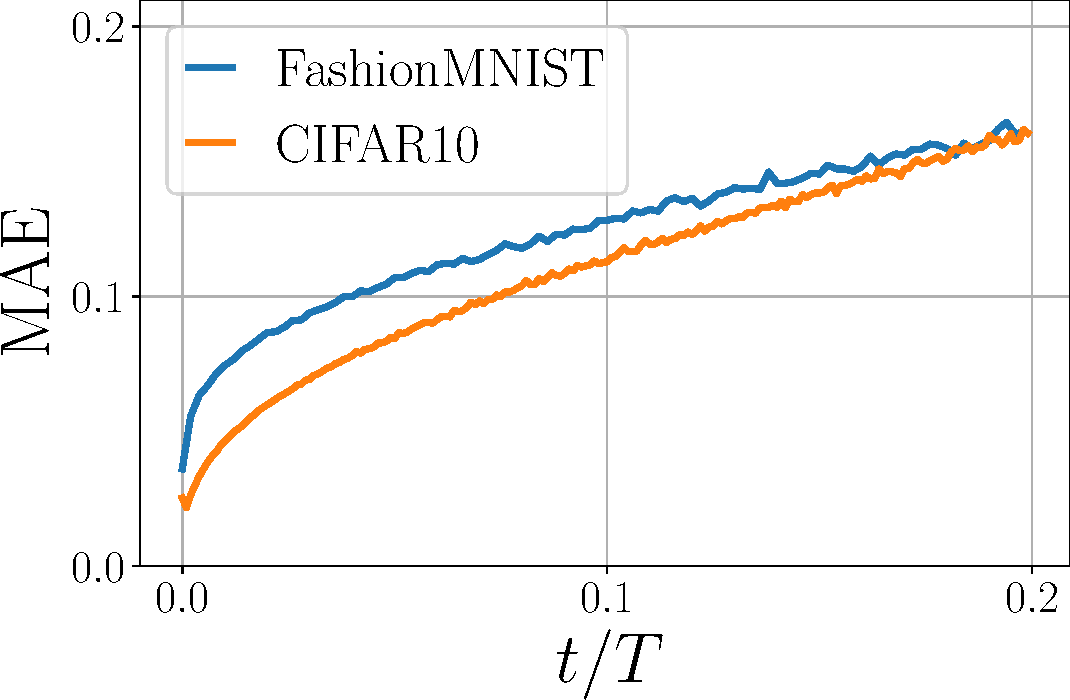
\includegraphics[width=0.4\textwidth]{pics/4_daed/experiments/MAE_step.pdf} &
        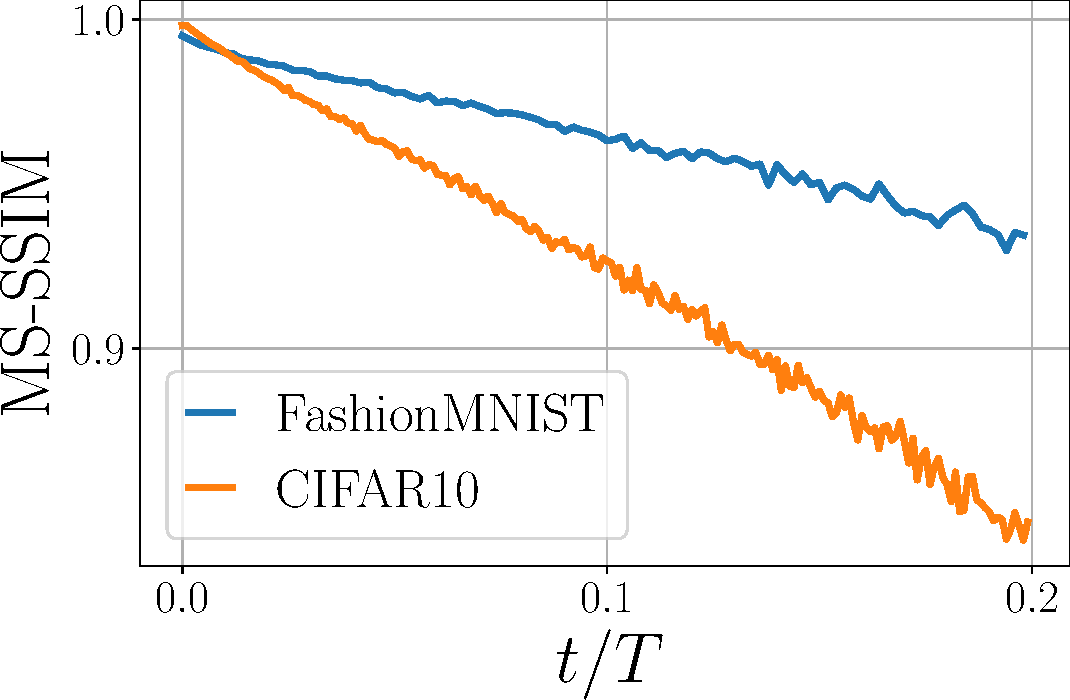
\includegraphics[width=0.4\textwidth]{pics/4_daed/experiments/MSSSIM_step.pdf} \\
    \end{tabular}
%    \end{adjustbox}
    \caption{The averaged reconstruction error calculated using (\textit{left}) the MAE, and (\textit{right}) the MS-SSIM at different steps of a DDGM.}
    \label{fig:reconstruction_error_analysis}
    \vspace*{\baselineskip}
     \end{figure}
%\end{wrapfigure}


We present the values on two datasets (FashionMNIST and CIFAR10) for the first 20\% of steps. Apparently, after around $10\%$ of the steps, the reconstruction error starts growing, and the MAE increases linearly above $0.1$ (i.e., about $6\%$ of error per pixel). At the same time, the MS-SSIM drops below $0.9-0.95$ (i.e., the discrepancy between original images and reconstructions becomes perceptually evident). This observation might suggest that DDGMs could be roughly divided into two parts: a fraction of steps of a DDGM (e.g., first $10\%$ of the steps) constitute a \textit{denoiser} that turns a corrupted image into a clear image, and the remaining steps of the DDGM are responsible for turning noise into a noisy structure (a corrupted image), i.e., a \textit{generator} that generates meaningful patterns. In other words, we claim that DDGM can be interpreted as a composition of a denoiser and a generator, but the boundary between those two parts is fluid. Moreover, the denoiser gradually removes the noise in a generative manner (i.e., by sampling $\rvx_{t-1} \sim p(\rvx_{t-1}|\rvx_t)$).


\paragraph{DDGMs as hierarchical VAEs} In this paper, we postulate that DDGMs could be seen as a composition of parts that serve different purposes. We can get additional insight into our claim by noticing a close connection between DDGMs and hierarchical VAEs. As presented in \cite{huang2021variational,kingma2021variational,tomczak2022deep}, if we treat all $\rvx_t$'s with $t>0$ as latents, and see the forward diffusion process as a composition of (non-trainable) variational posteriors, DGGMs become a specific formulation of hierarchical VAEs. On the other hand, we can start with a VAE with a single latent variable, $\rvx_1$, for which the variational lower bound is equal to:
\begin{equation}
    \ln p(\rvx_0) \geq \mathbb{E}_{\rvx_1 \sim q(\rvx_1 | \rvx_0)}\left[\ln p(\rvx_0|\rvx_1)\right] - D_{\text{KL}}[q(\rvx_1 | \rvx_0)||p(\rvx_1)].
\end{equation}
Then, similarly to \cite{vahdat2021score,wehenkel2021diffusion}, the marginal $p(\rvx_1)$ could be further modeled by a DDGM. By keeping the dimensionality of $\rvx_1$ the same as $\rvx_0$, and taking the variational posterior $q(\rvx_1 | \rvx_0)$ to be fixed and part of the forward diffusion, we get the DDGM model. This perspective of combining a VAE with a DDGM opens new possibilities for developing hybrid models.

\section{\ours{}: Denoising Auto-Encoder with Diffusion}

In this work, we propose a specific combination that distinctly splits the DDGM into generative and denoising parts. As noted in the previous section, the signal in the forward diffusion process is the strongest within the first $10-20\%$ of steps, and, thus, we postulate to perceive this first part of a DDGM as a denoiser. 
Together with the observation about the combination of a VAE with a DDGM-based prior, we consider turning a denoising auto-encoder into a generative model as presented in Figure~\ref{fig:teaser}. We bring a DDGM-based part into DAE for generating corrupted images. The resulting objective is the following:
\begin{align}
    \overline{\ell}(\rvx_0;\varphi, \theta) &= \mathbb{E}_{\rvx_1 \sim q(\rvx_1 | \rvx_0)}\left[\ln p\left(\rvx_0 | f_{\varphi}\left(\rvx_1\right)\right) + \ln p_{\theta}(\rvx_1)\right] \label{eq:daed_1}\\ 
    &\geq \underbrace{\mathbb{E}_{\rvx_1 \sim q(\rvx_1 | \rvx_0)}\left[\ln p\left(\rvx_0 | f_{\varphi}\left(\rvx_1\right)\right)\right]}_{\ell_{\text{DAE}}(\rvx_0;\varphi)} \\
    &\quad + \underbrace{\mathbb{E}_{q(\rvx_2, \ldots , \rvx_T | \rvx_1)} \left[ \frac{\ln p_{\theta}(\rvx_1, \ldots, \rvx_T)}{q(\rvx_1, \ldots , \rvx_T | \rvx_0)} \right]}_{\ell_{\text{D}}(\rvx_0;\theta)} \label{eq:dead_2},
\end{align}
where in (\ref{eq:dead_2}) we introduce additional latent variables and the variational posterior over them, that yields the variational lower bound. We call the resulting model \textit{DAE with a Diffusion}, or DEAD for short. In a sense, DAED is a DDGM with distinct parameterizations of the part between $\rvx_0$ and $\rvx_1$, and the part for the remaining $\rvx$'s. Thus, DEAD is almost identical to a DDGM, but there are the following differences:
% \begin{itemize}[leftmargin=*]
%     \item We can control the amount of noise in $q(\rvx_1|\rvx_0)$. It can correspond to the first step of the forward diffusion model, or we can introduce more noise at once that would correspond to several steps in the DDGM.
%     \item We use two different parameterizations, namely, an auto-encoder (e.g., a U-Net architecture) for $f_{\varphi}(\cdot)$ and a separate, shared U-Net for modeling the DDGM from $\rvx_1$ to $\rvx_T$. Since there are two neural networks, the lower bound to the objective $\overline{\ell}$ is in fact a composition of two objectives with disjunctive parameters, namely, the objective for the \textit{denoiser}, $\ell_{\text{DAE}}$, and the objective for the \textit{generator} (i.e., the diffusion-based generative model), $\ell_{\text{D}}$.
%     \item In the \ours{}, we introduce the \textit{denoiser} explicitly and make a clear distinction between the denoising and the generating parts while, as discussed earlier, this boundary is rather fluid in DDGMs. By introducing \ours{}, we can analyze what happens if we distinctly divide those two aspects with two separate parametrizations.
% \end{itemize}
\textbf{(i)} We can control the amount of noise in $q(\rvx_1|\rvx_0)$. It can correspond to the first step of the forward diffusion model, or we can introduce more noise at once that would correspond to several steps in the DDGM. \textbf{(ii)} We use two different parameterizations, namely, an auto-encoder (e.g., a U-Net architecture) for $f_{\varphi}(\cdot)$ and a separate, shared U-Net for modeling the DDGM from $\rvx_1$ to $\rvx_T$. Since there are two neural networks, the lower bound to the objective $\overline{\ell}$ is in fact a composition of two objectives with disjunctive parameters, namely, the objective for the \textit{denoiser}, $\ell_{\text{DAE}}$, and the objective for the \textit{generator} (i.e., the diffusion-based generative model), $\ell_{\text{D}}$. \textbf{(iii)} In the \ours{}, we introduce the \textit{denoiser} explicitly and make a clear distinction between the denoising and the generating parts while, as discussed earlier, this boundary is rather fluid in DDGMs. By introducing \ours{}, we can analyze what happens if we distinctly divide those two aspects with two separate parametrizations.

Moreover, we hypothesize that the resulting model may better generalize across various data distributions due to decoupling the parameterization of the denoiser and the generator. The training dataset may bias a single, shared parameterization in a DDGM, and while denoising an image from a different domain, it may add some artifacts from the source. While with two distinct parameterizations, there might be a lower chance for that. We evaluate this hypothesis in the experiments. 